\documentclass{article}
\usepackage[utf8]{inputenc}

\title{CS 107 Review Questions: LaTeX Helper Document}
\author{Randy Dang}
\date{January 2, 2024}

\usepackage{natbib}
\usepackage{graphicx}

\usepackage{amsmath}
\usepackage{fullpage}
\usepackage{hyperref}
\hypersetup{
    colorlinks=true,
    linktoc=all, 
    linkcolor=blue,
    urlcolor=blue
}
\usepackage{tikz}
\usetikzlibrary{automata,positioning}

\begin{document}

\maketitle

\section{Question 6}

\subsection{Option 1}

\bigskip

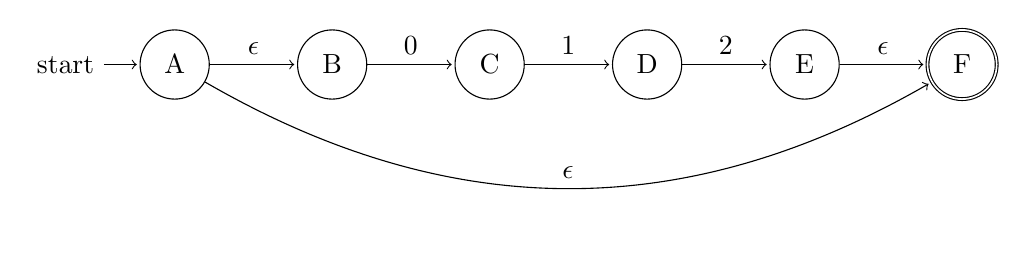
\begin{tikzpicture}[shorten >=1pt,node distance=2cm,on grid,auto]
    \node[state, initial] (q_1) {A};
    \node[state] [right=of q_1] (q_2) {B};
    \node[state] [right=of q_2] (q_3) {C};
    \node[state] [right=of q_3] (q_4) {D};
    \node[state] [right=of q_4] (q_5) {E};
    \node[state, accepting] [right=of q_5] (q_6) {F};

    \path[->]
    (q_1) edge node {$\epsilon$} (q_2)
    (q_2) edge node {0} (q_3)
    (q_3) edge node {1} (q_4)
    (q_4) edge node {2} (q_5)
    (q_5) edge node {$\epsilon$} (q_6)
    (q_1) edge [bend right=30] node {$\epsilon$} (q_6)
    ;
\end{tikzpicture}

\bigskip

\subsection{Option 2}

\bigskip

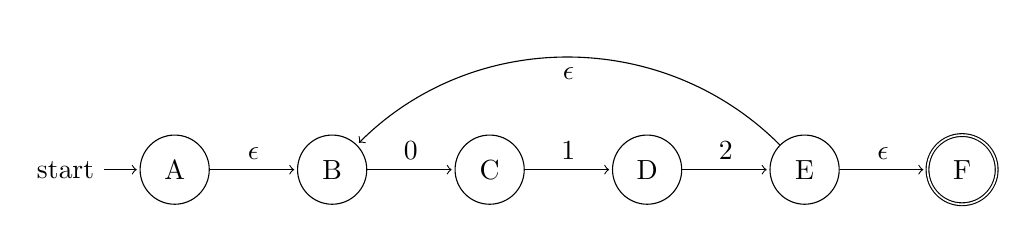
\begin{tikzpicture}[shorten >=1pt,node distance=2cm,on grid,auto]
    \node[state, initial] (q_1) {A};
    \node[state] [right=of q_1] (q_2) {B};
    \node[state] [right=of q_2] (q_3) {C};
    \node[state] [right=of q_3] (q_4) {D};
    \node[state] [right=of q_4] (q_5) {E};
    \node[state, accepting] [right=of q_5] (q_6) {F};

    \path[->]
    (q_1) edge node {$\epsilon$} (q_2)
    (q_2) edge node {0} (q_3)
    (q_3) edge node {1} (q_4)
    (q_4) edge node {2} (q_5)
    (q_5) edge node {$\epsilon$} (q_6)
    (q_5) edge [bend right=45] node {$\epsilon$} (q_2)
    ;
\end{tikzpicture}

\bigskip

\subsection{Option 3}

\bigskip

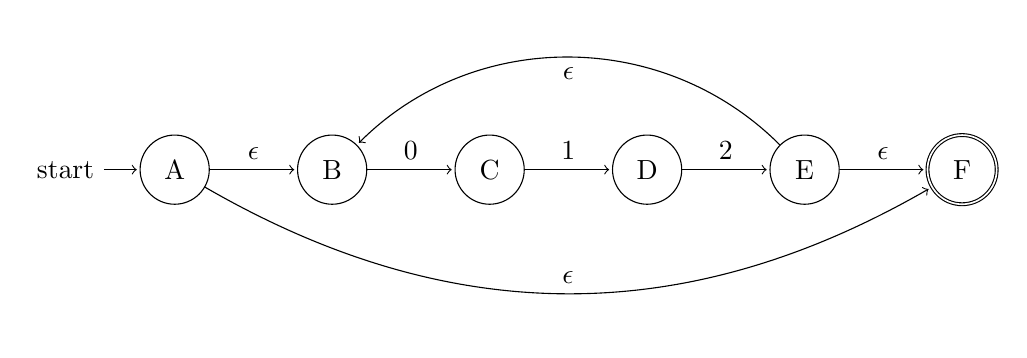
\begin{tikzpicture}[shorten >=1pt,node distance=2cm,on grid,auto]
    \node[state, initial] (q_1) {A};
    \node[state] [right=of q_1] (q_2) {B};
    \node[state] [right=of q_2] (q_3) {C};
    \node[state] [right=of q_3] (q_4) {D};
    \node[state] [right=of q_4] (q_5) {E};
    \node[state, accepting] [right=of q_5] (q_6) {F};

    \path[->]
    (q_1) edge node {$\epsilon$} (q_2)
    (q_2) edge node {0} (q_3)
    (q_3) edge node {1} (q_4)
    (q_4) edge node {2} (q_5)
    (q_5) edge node {$\epsilon$} (q_6)
    (q_5) edge [bend right=45] node {$\epsilon$} (q_2)
    (q_1) edge [bend right=30] node {$\epsilon$} (q_6)
    ;
\end{tikzpicture}

\bigskip

\subsection{Option 4}

\bigskip 

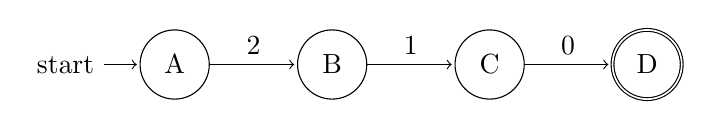
\begin{tikzpicture}[shorten >=1pt,node distance=2cm,on grid,auto]
    \node[state, initial] (q_1) {A};
    \node[state] [right=of q_1] (q_2) {B};
    \node[state] [right=of q_2] (q_3) {C};
    \node[state, accepting] [right=of q_3] (q_4) {D};

    \path[->]
    (q_1) edge node {2} (q_2)
    (q_2) edge node {1} (q_3)
    (q_3) edge node {0} (q_4)
    ;
\end{tikzpicture}

\bigskip 

\end{document}
